\documentclass[11pt]{article}
\usepackage{geometry, titlesec}
\usepackage[parfill]{parskip}
\usepackage[italicdiff]{physics}
\usepackage{amsfonts, amsthm}
\usepackage[cm]{fullpage}
\usepackage{fancyhdr}
\usepackage{enumitem}
\usepackage{xcolor, soul}
\usepackage{graphicx}
\usepackage[export]{adjustbox}
\usepackage{siunitx}
%\allowdisplaybreaks

\renewcommand{\thesubsection}{\thesection.\alph{subsection}}
\setenumerate[1]{label={(\alph*)}}

\makeatletter
\renewcommand*\env@cases[1][1.2]{%
  \let\@ifnextchar\new@ifnextchar
  \left\lbrace
  \def\arraystretch{#1}%
  \array{@{}l@{\quad}l@{}}%
}
\makeatother
 
\renewcommand{\footrulewidth}{.2pt}
%\setlist[enumerate]{leftmargin=*}
\pagestyle{fancy}
\fancyhf{}
\rhead{Physics 132-B}
\lhead{\textbf{Homework 5 Solutions}}
%\rhead{A--De Discussion}
\setlength{\headheight}{11pt}
\setlength{\headsep}{11pt}
\setlength{\footskip}{24pt}
\lfoot{\today}
\rfoot{\thepage}

\titleformat{\subsection}[runin]{\normalfont\large\bfseries}{\thesubsection}{1em}{}
\newcommand{\refeq}[1]{(\ref{#1})}

\newcommand{\beq}{\begin{equation*}}
\newcommand{\eeq}{\end{equation*}}

\newcommand{\beqn}{\begin{equation}}
\newcommand{\eeqn}{\end{equation}}

\newcommand{\blg}{\begin{align*}}
\newcommand{\elg}{\end{align*}}

\makeatletter
\renewcommand*\env@matrix[1][*\c@MaxMatrixCols c]{%
  \hskip -\arraycolsep
  \let\@ifnextchar\new@ifnextchar
  \array{#1}}
\makeatother


\newenvironment{statement}
{
%    \color{gray}
    \ignorespaces
}
{
%    \smallskip
}

\newenvironment{problem}
{
    \color{darkgray}
    \ignorespaces
}

\newenvironment{solution}
{
    \paragraph{Solution.}
    \ignorespaces
}
{
    \bigskip
}

\renewcommand{\vec}[1]{\mathbf{#1}}
\renewcommand{\theequation}{\Alph{equation}}


\begin{document}

\newcommand{\Vab}{V_{ab}}
\newcommand{\cE}{\mathcal{E}}
\newcommand{\sicE}{\SI{12.0}{\volt}}
\newcommand{\sir}{\SI{0.40}{\ohm}}
\newcommand{\siP}{\SI{80.0}{\watt}}
\newcommand{\qimplies}{\quad\implies\quad}
	

\paragraph{Problem 25.58}
\begin{problem}
	A resistor with resistance $R$ is connected to a battery that has emf {\sicE} and internal resistance $r = \sir$.  For what two values of $R$ will the power in the resistor be {\siP}?
\end{problem}

\begin{solution}
	We can think of the battery's internal resistance as another resistor of resistance $r$ connected in series.
	
	\vspace{1.5in}

	The power $P$ delivered to the resistor of resistance $R$ is
	\beqn \tag{25.18} \label{25.18}
		P = I^2 R,
	\eeqn
	where $I$ is the current through the resistor.  We have a one-loop circuit, so the current through all elements is the same.  We can easily find $I$ using Kirchhoff's loop rule,
	\beq
		\sum V = 0. \tag{26.6}
	\eeq
	Let's start at the battery and work counterclockwise as indicated in the diagram.  We get
	\beq
		0 = \cE - I r - I R
		\qimplies
		\cE = I (R + R)
		\qimplies
		I = \frac{\cE}{R + r}.
	\eeq
	Now we can substitute this result into \refeq{25.18} and solve for $R$:
	\begin{align*}
		P = \frac{\cE^2}{(R + r)^2} R
		&\qimplies
		\cE^2 R = P (R^2 + 2 R r + r^2)
		\qimplies
		0 = P R^2 + (2P r - \cE^2) R + P r^2 \\
		&\qimplies
		R = \frac{\cE^2 - 2 P r \pm \sqrt{(2P r - \cE^2)^2 - 4 P^2 r^2}}{2 P}.
	\end{align*}
	Plugging in our numerical values for $r$, $P$, and $\cE$, and recalling that $\SI{1}{\watt} = \SI{1}{\square\volt\per\ohm}$, we get
	\begin{align*}
		R &= \frac{(\sicE)^2 - 2 (\siP) (\sir) \pm \sqrt{[2 (\siP) (\sir) - (\sicE)^2]^2 - 4 (\siP)^2 (\sir)^2}}{2 (\siP)} \\[1.5ex]
		&= \frac{\SI{80.0}{\square\volt} - \pm \sqrt{(\SI{80}{\square\volt})^2 - (\SI{64}{\square\volt})}}{\SI{160}{\square\volt\per\ohm}}
		= \frac{\SI{80.0}{\square\volt} \pm \sqrt{\SI{2306}{\volt^4}}}{\SI{160}{\square\volt\per\ohm}}
		= \frac{80.0 \pm 48.0}{160} \,\si{\ohm}
		= (0.50 \pm 0.30) \,\si{\ohm}.
	\end{align*}
	So the two possible resistances are
	{\color{blue} \begin{align*}
		R &= \SI{0.80}{\ohm}, &
		R &= \SI{0.20}{\ohm}.
	\end{align*}}
\end{solution}

\clearpage



\newcommand{\Iq}{I_1}
\newcommand{\Iw}{I_2}
\newcommand{\Ie}{I_3}
\newcommand{\Sohm}[1]{\SI{#1}{\ohm}}
\newcommand{\Svolt}[1]{\SI{#1}{\volt}}
\newcommand{\Samp}[1]{\SI{#1}{\ampere}}

\begin{minipage}[l]{0.7\textwidth}
\paragraph{Exercise 26.26}
\begin{problem}
	In the circuit shown in \textbf{Fig.~E26.26}, find \medskip
	\begin{enumerate}
		\item the current in each branch, and \medskip
		\item the potential difference $\Vab$ of point $a$ relative to point $b$.
	\end{enumerate}
\end{problem}
\end{minipage}%
\hspace{0.05\textwidth}%
\begin{minipage}{0.25\textwidth}
	\center 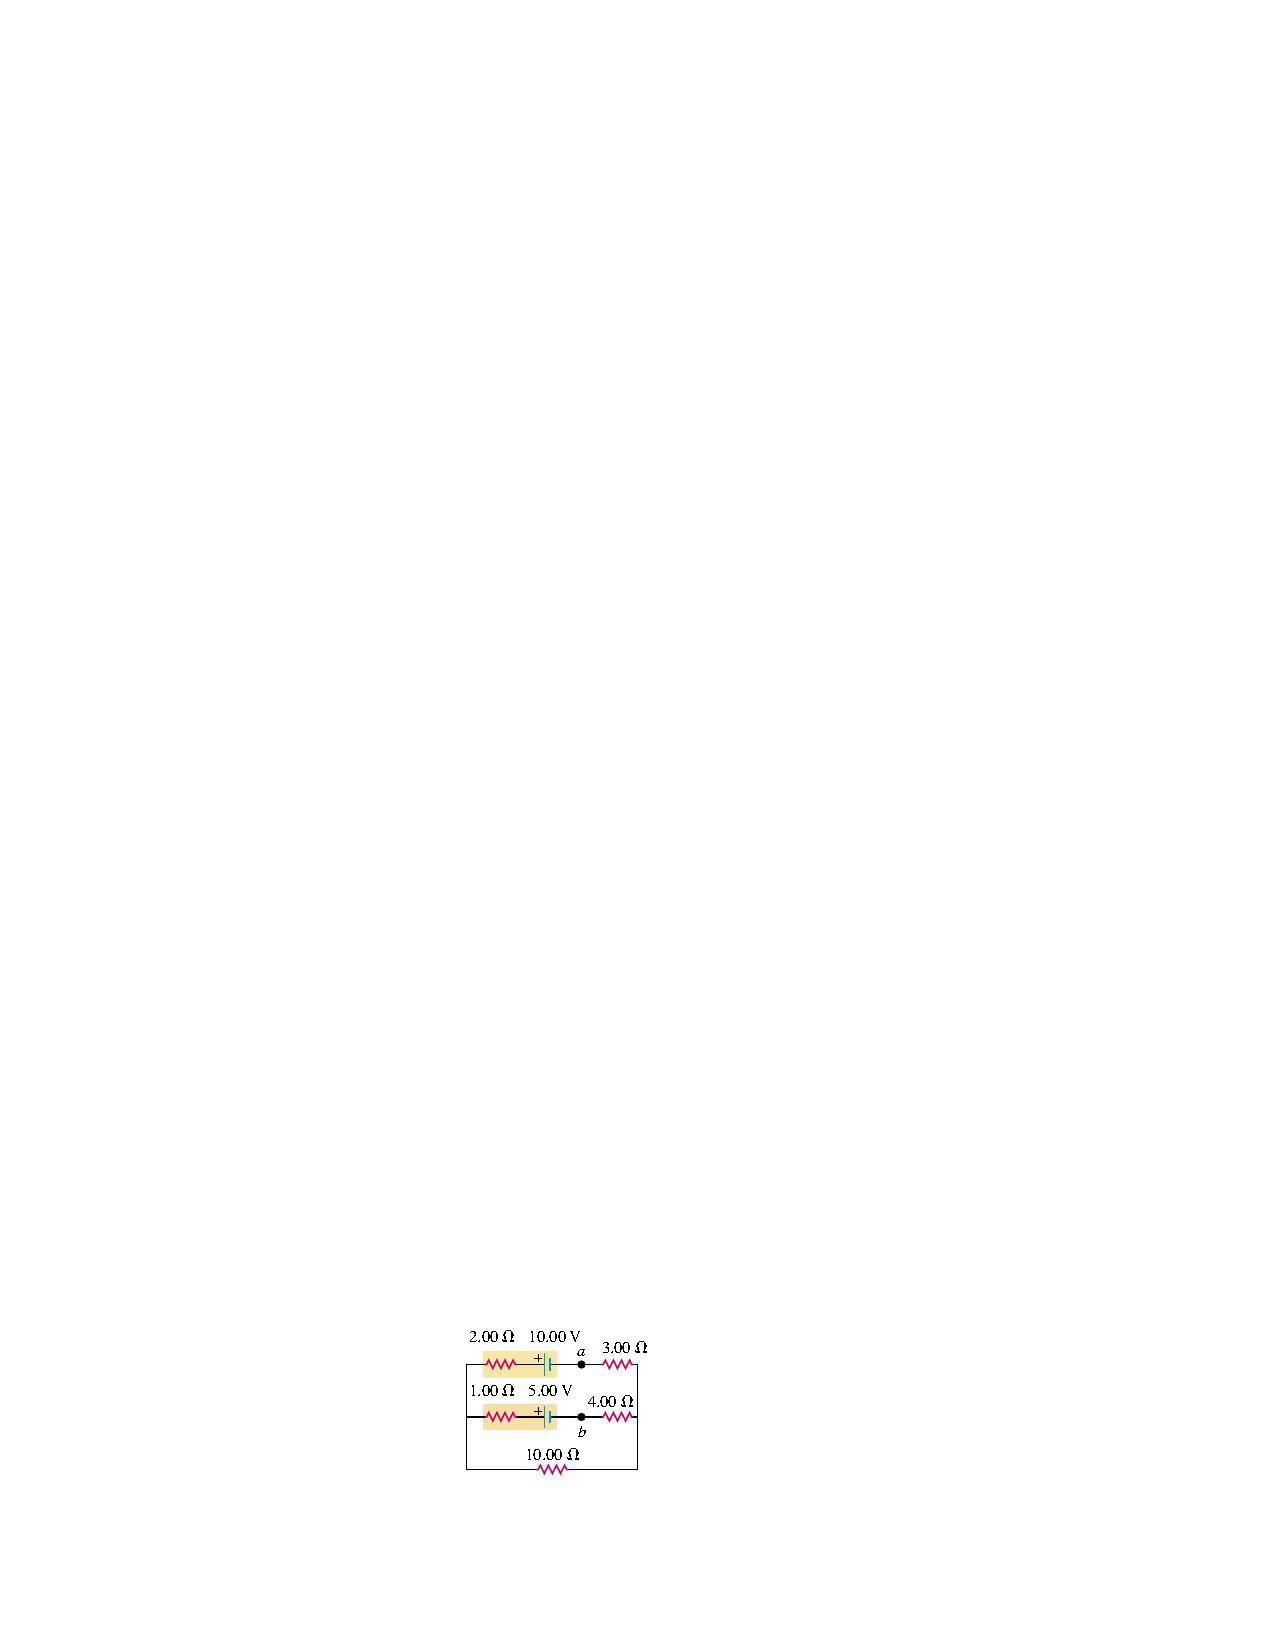
\includegraphics{E26-26}
	\center \textbf{Figure E26.26}
\end{minipage}


\begin{solution}
 	For this problem we need to use Kirchhoff's rules:
	\begin{align}
		\sum I &= 0 & &\text{(junction rule)}, \tag{26.5} \label{26.5} \\
		\sum V &= 0 & &\text{(loop rule)}. \tag{26.6} \label{26.6}
	\end{align}
	
	\begin{enumerate}
		\item Let $\Iq$ be the current through the top branch, $\Iw$ the current through the middle branch, and $\Ie$ the current through the bottom branch.  Let's choose all three currents to be flowing to the left.
		
		\vspace{3in}
		
		
		Then applying the junction rule to the junction on the left~(shown in red) gives us
		\beqn \label{junction}
			0 = \Iq + \Iw + \Ie,
		\eeqn
		which would not make sense if we had chosen the directions of all three currents correctly.  But the currents whose direction we have chosen incorrectly will just end up being negative in our solution.
		
		
		Now let's apply the loop rule to the top and the bottom loops, and move through each counterclockwise, starting at the battery.  For the top loop,
		\beq
			0 = \Svolt{10} - (\Sohm{2}) \Iq + (\Sohm{1}) \Iw - \Svolt{5} + (\Sohm{4}) \Iw - (\Sohm{3}) \Iq
			\qimplies
			\Svolt{5} = (\Sohm{5}) \Iq - (\Sohm{5}) \Iw,
		\eeq
		which simplifies to
		\beqn \label{top}
			\Samp{1} = \Iq - \Iw,
		\eeqn
		where we have just divided by $\Sohm{5}$, since $\SI{1}{\volt} = \SI{1}{\ohm\ampere}$.  For the bottom loop,
		\beq
			0 = \Svolt{5} - (\Sohm{1}) \Iw + (\Sohm{10}) \Ie - (\Sohm{4}) \Iw
			\qimplies
			\Svolt{5} = (\Sohm{5}) \Iw - (\Sohm{10}) \Ie,
		\eeq
		which simplifies to
		\beqn \label{bottom}
			\Samp{1} = \Iw - 2 \Ie.
		\eeqn
		
		Now we have the three equations~\refeq{junction}, \refeq{top}, and \refeq{bottom} in three unknowns, which you can solve using your favorite method.  If we want to solve them algebraically, we can begin by solving \refeq{junction} for $\Iq$, which gives us
		\beq
			\Iq = - \Iw - \Ie.
		\eeq
		Now we can feed this into \refeq{top} and solve for $\Iw$:
		\beq
			\Samp{1} = -\Iw - \Ie - \Iw = -2 \Iw - \Ie
			\qimplies
			\Iw = -\frac{\Ie + \Samp{1}}{2}
			= -\frac{\Ie}{2} - \frac{1}{2}\,\si{\ampere}.
		\eeq
		Substituting this expression into \refeq{bottom}, we get
		\beq
			\Samp{1} = -\frac{\Ie}{2} - \frac{1}{2}\,\si{\ampere} - 2 \Ie
			\qimplies
			\frac{5 \Ie}{2} = -\frac{3}{2}\,\si{\ampere}
			\qimplies
			\Ie = \frac{3}{5}\,\si{\ampere}.
		\eeq
		Now we can plug this result for $\Ie$ into \refeq{bottom} to find $\Iw$:
		\beq
			\Samp{1} = \Iw + 2 \frac{3}{5}\,\si{\ampere} = \Iw + \frac{6}{5}\,\si{\ampere}
			\implies
			\Iw = -\frac{1}{5}\,\si{\ampere}.
		\eeq
		Finally, we can plug this result for $\Iw$ into \refeq{top} to get $\Iq$:
		\beq
			\Samp{1} = \Iq + \frac{1}{5}\,\si{\ampere}
			\qimplies
			\Iq = \frac{4}{5}\,\si{\ampere}.
		\eeq
		As it turns out, both $\Iw$ and $\Ie$ are in the direction opposite of what we guessed.  Gathering all of our results, we have
		{\color{blue} \begin{align*}
			\text{Top branch: }& \Samp{0.800} \text{ (to the left)}, \\
			\text{Middle branch: }& \Samp{0.200} \text{ (to the right)}, \\
			\text{Bottom branch: }& \Samp{0.600} \text{ (to the right)}.
		\end{align*}}

		For a tricky system of three or more equations, it might be easier to use Gaussian elimination instead.  The matrix equation is
		\beq
			\mqty[ 1 & 1 & 1 \\
				1 & -1 & 0 \\
				0 & 1 & -2 ]
				\mqty[ \Iq \\ \Iw \\ \Ie ]
				= \mqty[ 0 \\ 1 \\ 1 ],
		\eeq
		which can be solved as follows:
		\beq
			\begin{bmatrix}[c c c | c]
				1 & 1 & 1 & 0 \\
				1 & -1 & 0 & 1 \\
				0 & 1 & -2 & 1
			\end{bmatrix}
			\sim
			\begin{bmatrix}[c c c | c]
				1 & -1 & 0 & 1 \\
				0 & 1 & -2 & 1 \\
				1 & 1 & 1 & 0
			\end{bmatrix}
			\sim
			\begin{bmatrix}[c c c | c]
				1 & 0 & -2 & 2 \\
				0 & 1 & -2 & 1 \\
				0 & 2 & 1 & -1
			\end{bmatrix}
			\sim
			\begin{bmatrix}[c c c | c]
				1 & 0 & -2 & 2 \\
				0 & 1 & -2 & 1 \\
				0 & 0 & 5 & -3
			\end{bmatrix}
			\sim
			\begin{bmatrix}[c c c | c]
				1 & 0 & 0 & 4/5 \\
				0 & 1 & 0 & -1/5 \\
				0 & 0 & 1 & -3/5
			\end{bmatrix},
		\eeq
		which is the same as what we got through algebraic substitution.
		
		\vfill
		
		\item We can find the potential difference between points $a$ and $b$ by moving counterclockwise through the top loop, similar to applying the loop rule in (a).  But now we start at $b$ and end on $a$:
		\beq
			\Vab = (\Sohm{4}) \Iw - (\Sohm{3}) \Iq
			= (\Sohm{4.00}) (-\Samp{0.200}) - (\Sohm{3.00}) (\Samp{0.800})
			= {\color{blue} \Svolt{32.0}}.
		\eeq
	\end{enumerate}
\end{solution}



\clearpage

\newcommand{\Req}{R_\text{eq}}
\newcommand{\Rtot}{R_\text{tot}}

\begin{minipage}[l]{0.65\textwidth}
\paragraph{Exercise 26.29}
\begin{problem}
	In the circuit shown in \textbf{Fig.~E26.29} the batteries have negligible internal resistance and the meters are both idealized.  With the switch $S$ open, the voltmeter reads \SI{15.0}{\volt}. \medskip
	\begin{enumerate}
		\item Find the emf $\cE$ of the battery. \medskip
		\item What will the ammeter read when the switch is closed?
	\end{enumerate}
\end{problem}
\end{minipage}%
\hspace{0.05\textwidth}%
\begin{minipage}{0.3\textwidth}
	\center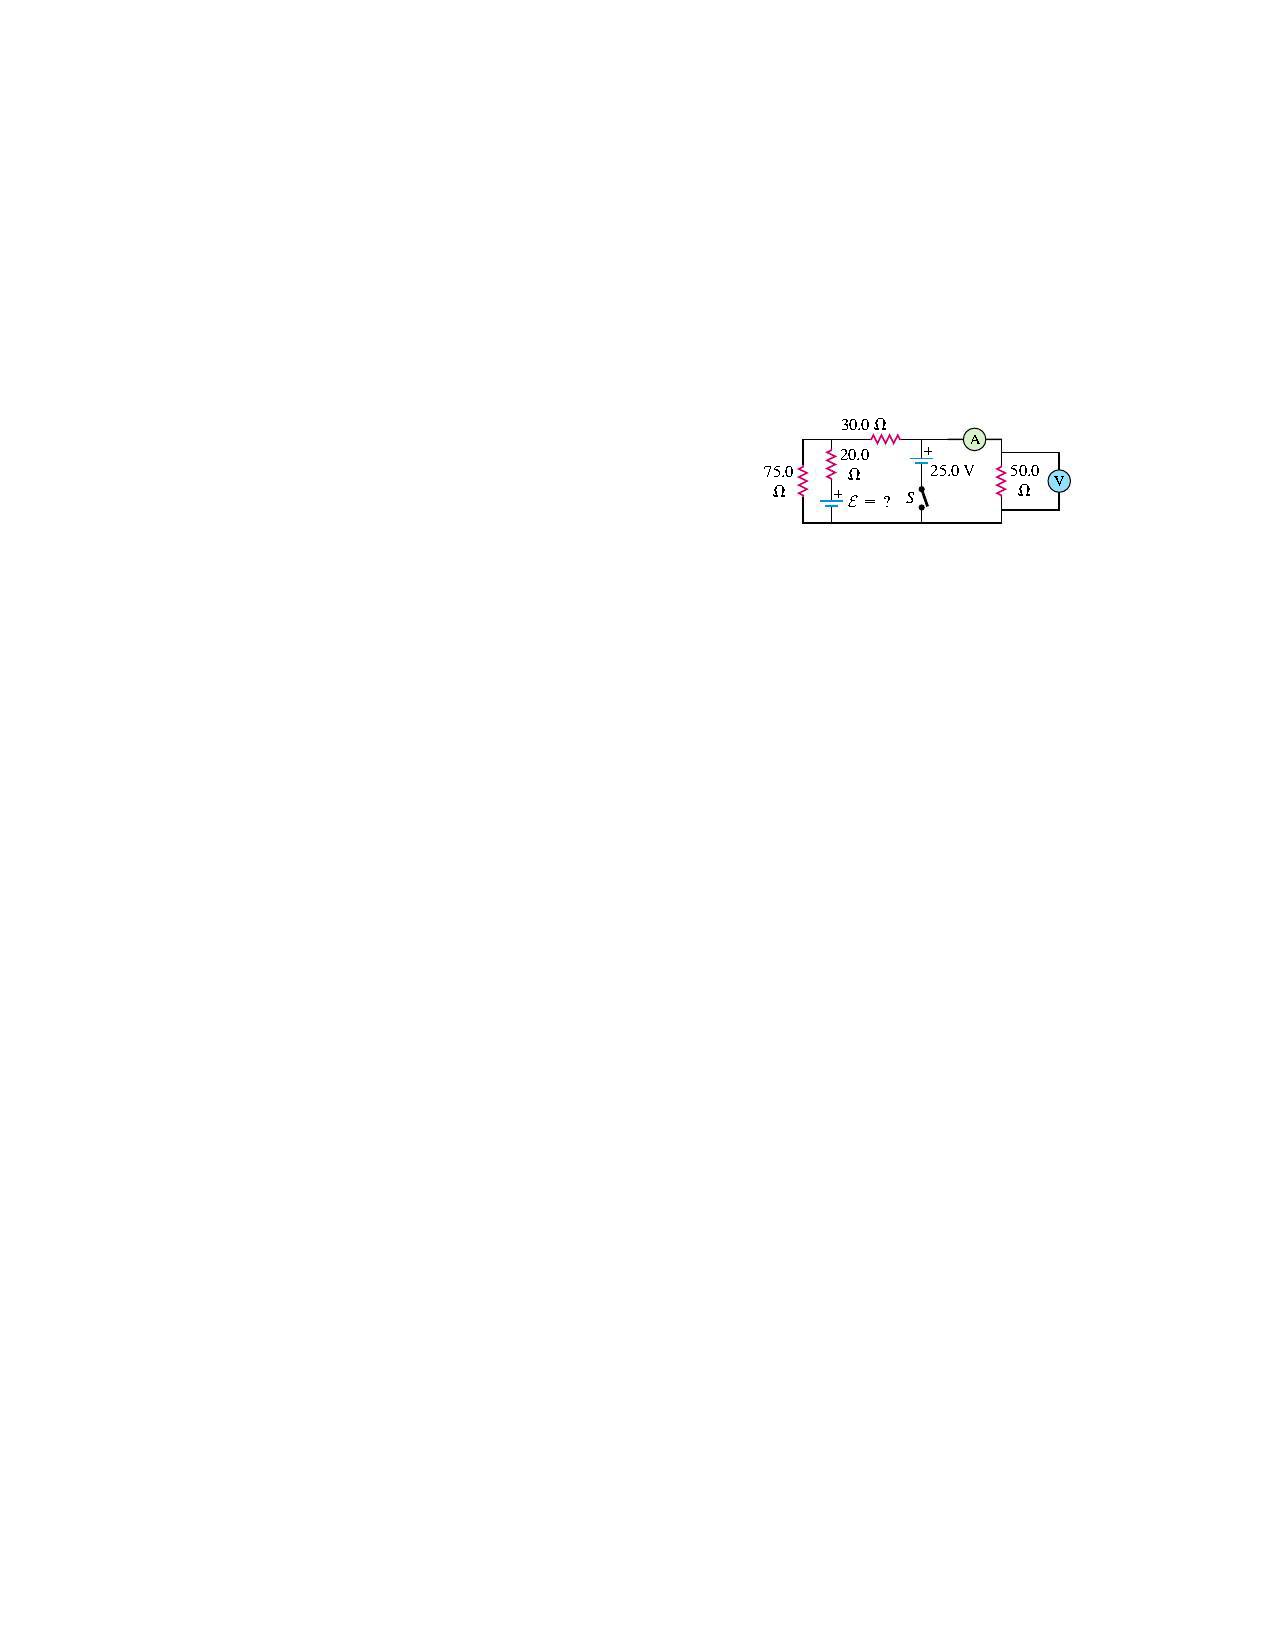
\includegraphics{E26-29}
	\center \textbf{Figure E26.29}
\end{minipage}

\begin{solution}
	\begin{enumerate}
		\item We need to simplify the circuit to the point that we know the current through the battery and the single equivalent resistance connected to it.  When the switch is open, we can ignore the branch of the circuit with the \Svolt{25} battery.
		
		\vspace{1.5in}
		
		Let's begin with what we are given, which is the voltmeter reading.  Since the voltmeter is connected in parallel to the \Sohm{50} resistor, we know that the potential across this resistor is \Svolt{15}.  So we can use Ohm's law to find the current through this resistor:
		\beq
			V = I R
			\qimplies
			I_{\Sohm{50}} = \frac{\Svolt{15}}{\Sohm{50}}
			= \frac{3}{10}\,\si{\ampere}
			= \Samp{0.300}.
		\eeq
		This is the current through any components connected in series with the \Sohm{50} resistor, so it is also the current through their equivalent resistance.  The \Sohm{30} resistor is in series with the \Sohm{50} resistor, and their equivalent resistance is
		\beq
			{\Req}_1 = \Sohm{50} + \Sohm{30}
			= \Sohm{80.0}.
		\eeq
		
		\vspace{1.5in}
		
		The potential difference across ${\Req}_1$ can be found by using Ohm's law once more:
		\beq
			V_{\Sohm{80}} = I_{\Sohm{50}} {\Req}_1 = (\Samp{0.300}) (\Sohm{80.0}) = \Svolt{24.0}.
		\eeq
		This is also the potential difference across any components connected in parallel to ${\Req}_1$.  The \Sohm{75} resistor is connected in parallel, so we can find the current through it using Ohm's law:
		\beq
			I_{\Sohm{75}} = \frac{V_{\Sohm{80}}}{\Sohm{75}}
			= \frac{\Svolt{24.0}}{\Sohm{75.0}}
			= \Samp{0.320}.
		\eeq
		Applying Kirchhoff's junction rule to the top junction in the diagram just above, we can find the current through the branch of the circuit with the unknown emf $\cE$:
		\beq
			0 = I_\cE - I_{\Sohm{75}} - I_{\Sohm{80}}
			\qimplies
			I_\cE = \Samp{0.320} + \Samp{0.300}
			= \Samp{0.620}.
		\eeq
		Now that we know the current through the battery, we can simplify the circuit to just one equivalent resistance.  First adding the \Sohm{75} and \Sohm{80} resistors in parallel, we find
		\beq
			\frac{1}{{\Req}_2} = \frac{1}{\Sohm{75}} + \frac{1}{{\Req}_1}
			= \frac{1}{\Sohm{75}} + \frac{1}{\Sohm{80}}
			= \frac{31}{1200}\,\si{\per\ohm}
			\qimplies
			{\Req}_2 = \frac{1200}{31}\,\si{\ohm}
			= \Sohm{38.7}.
		\eeq
		
		\vspace{1.5in}
				
		Adding this in series with the \Sohm{20} resistor, we find
		\beq
			\Rtot = {\Req}_2 + \Sohm{20}
			= \Sohm{38.7} + \Sohm{20}
			= \Sohm{58.7}.
		\eeq
		
		\vspace{1.5in}
				
		Finally, we know that the potential across $\Rtot$ is the same as across the battery.  So Ohm's law tells us
		\beq
			\cE = I_\cE \Rtot
			= (\Samp{0.620}) (\Sohm{58.7})
			= {\color{blue} \Svolt{36.4}}.
		\eeq
		
		\vfill
		
		\item When the switch is closed, the \Sohm{50} resistor is connected in parallel to the \Svolt{25} battery, so the potential across the \Sohm{50} resistor is equal to \Svolt{25}.

		\vspace{1.5in}

		We can apply Ohm's law once more to find the current through the \Sohm{50} resistor, which is the same as the current through the ammeter connected in series:
		\beq
			I_A = \frac{\Svolt{25.0}}{\Sohm{50.0}}
			= {\color{blue} \Samp{0.500}}.
		\eeq
	\end{enumerate}
\end{solution}



\clearpage

\newcommand{\Qo}{Q_0}
\newcommand{\Vo}{V_0}
\newcommand{\Ceq}{C_\text{eq}}

\begin{minipage}[l]{0.75\textwidth}
\paragraph{Exercise 26.41}
\begin{problem}
	In the circuit shown in \textbf{Fig.~E26.41} both capacitors are initially charged to \SI{45.0}{\volt}. \medskip
	\begin{enumerate}
		\item How long after closing the switch $S$ will the potential across each capacitor be reduced to \SI{10.0}{\volt}, and \medskip
		\item what will be the current at that time? \medskip
	\end{enumerate}
\end{problem}
\end{minipage}%
\hspace{0.05\textwidth}%
\begin{minipage}{0.2\textwidth}
	\center 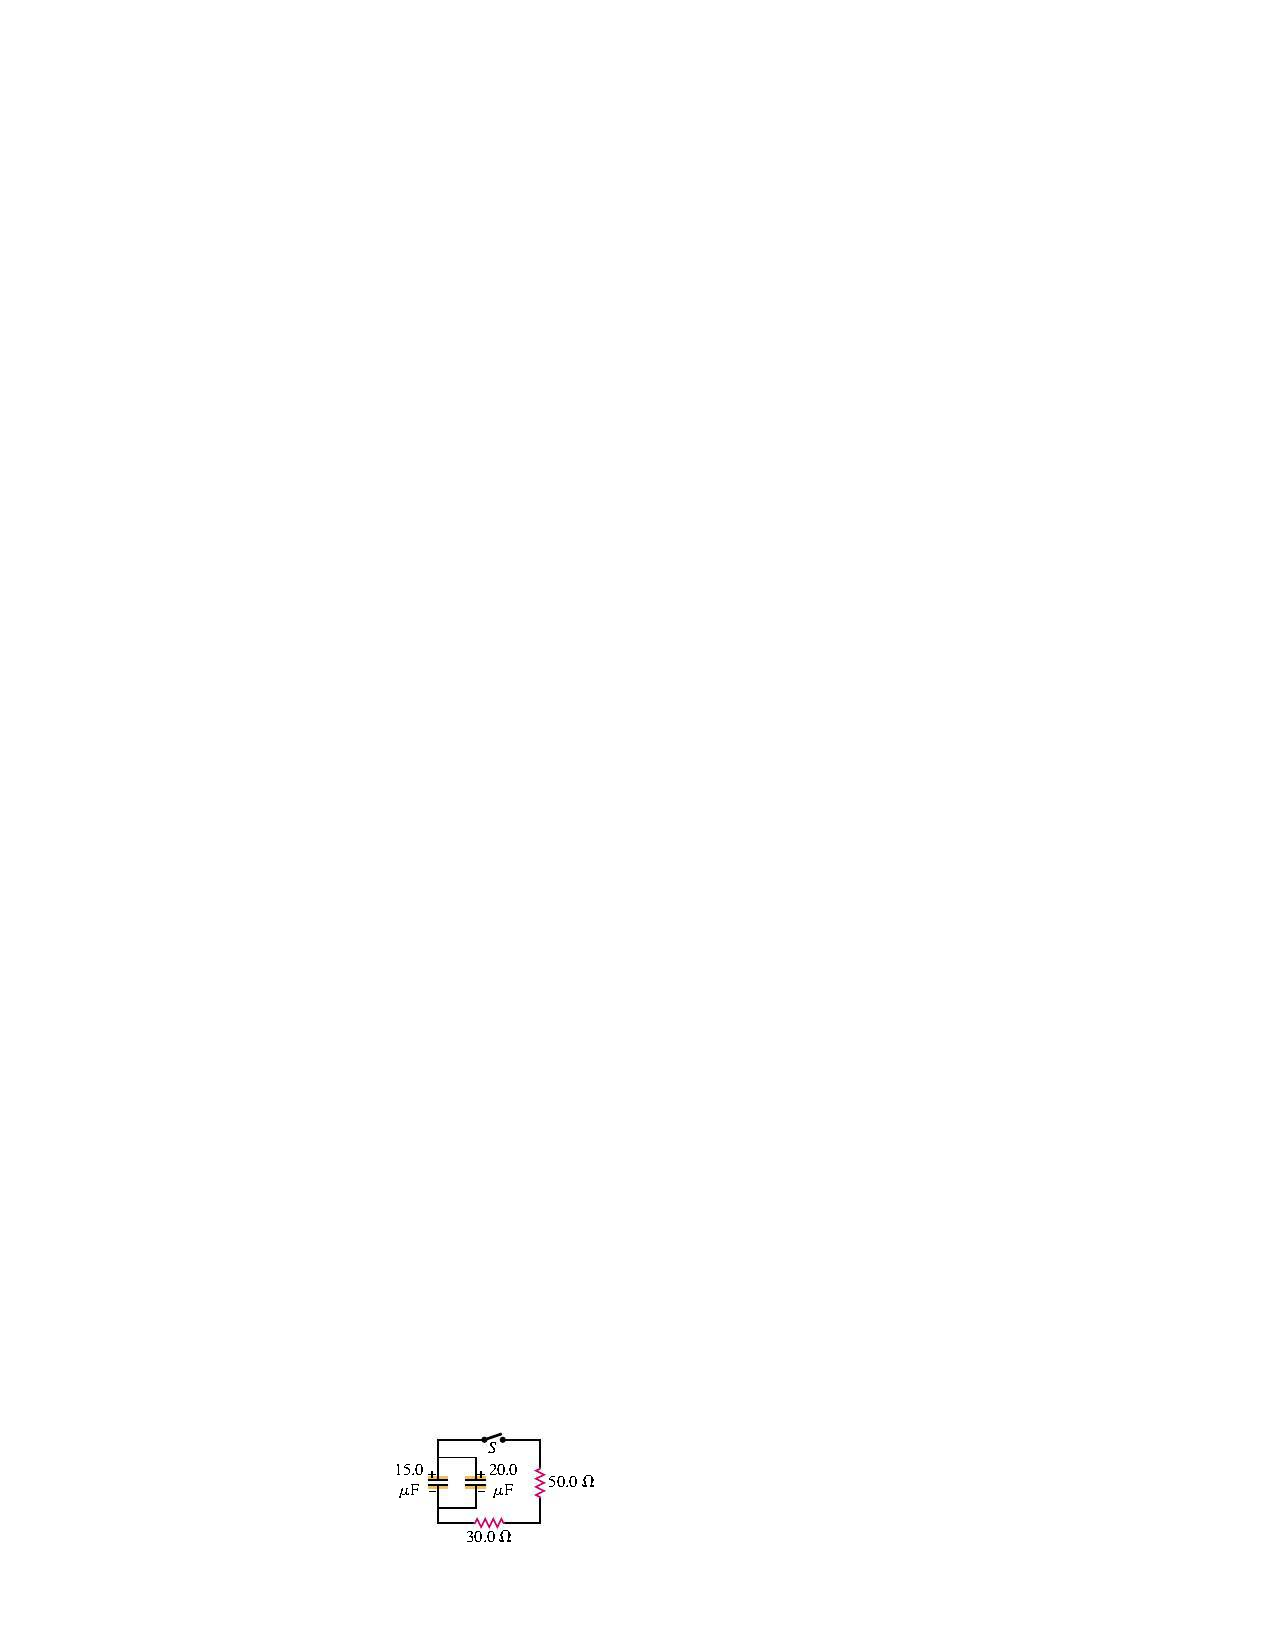
\includegraphics{E26-41}
	\center \textbf{Figure E26.41}
\end{minipage}

\begin{solution}
	This problem is about discharging capacitors.  The charge $q$ on a capacitor at time $t$ after closing an $RC$ circuit is given by
	\beqn \label{26.16} \tag{26.16}
		q = \Qo e^{-t / RC},
	\eeqn
	where $\Qo$ is the initial charge on the capacitor, $C$ is its capacitance, and $R$ is the resistance of the resistor connected to it in series.
	
	\begin{enumerate}
		\item The definition of capacitance is
		\beq
			C = \frac{Q}{V},
		\eeq
		where $Q$ is the charge on the capacitor and $V$ is the potential across it.  $C$ is a property of a given capacitor and does not change with time.  So we can use $Q = C V$ and the fact that $C$ is constant to write \refeq{26.16} in terms of $C$ and $V$:
		\beqn \tag{$*$} \label{Vt}
			v = \Vo e^{-t / RC},
		\eeqn
		where $v$ is the potential across the capacitor at time $t$.
		
		The capacitors in this problem are connected in parallel, so their equivalent capacitance is simply the sum of their individual capacitances:
		\beq
			\Ceq = \SI{15.0}{\micro\farad} + \SI{20.0}{\micro\farad}
			= \SI{35.0}{\micro\farad}.
		\eeq
		The resistors are connected in series, so their equivalent resistance is also just the sum:
		\beq
			\Req = \SI{30.0}{\ohm} + \SI{50.0}{\ohm}
			= \SI{80.0}{\ohm}.
		\eeq
		We can plug these values and our intended value of $v = \Svolt{10.0}$ into \refeq{Vt} to solve for the time $t$:
		\begin{align*}
			\Svolt{10.0} &= (\Svolt{45.0}) \exp(-\frac{t}{(\SI{80.0}{\ohm}) (\SI{35.0}{\micro\farad})})
			\qimplies
			\frac{2}{9} = \exp(-\frac{t}{\SI{2800}{\micro\second}})
			\qimplies
			-1.50 = -\frac{t}{\SI{2800}{\micro\second}} \\[1.5ex]
			&\qimplies
			t = \SI{4210}{\micro\second}
			= {\color{blue} \SI{4.21}{\milli\second}},
		\end{align*}
		where we have used the fact that $\SI{1}{\second} = \SI{1}{\ohm\farad}$.
		
		\vfill
		
		\item The current $i$ through a capacitor at a given time $t$ after the circuit is closed is given by
		\beq \tag{26.13}
			i = \frac{\Qo}{RC} e^{-t / RC}.
		\eeq
		From (a), we know that $\Qo / C = \Vo$, so we can write this as
		\beq
			i = \frac{\Vo}{R} e^{-t / RC}.
		\eeq
		Plugging in our $\Vo$, $\Req$, $\Ceq$, and $t$ that we found in (a), we have
		\beq
			i = \frac{\Svolt{45.0}}{\SI{80.0}{\ohm}} \exp(-\frac{\SI{4210}{\micro\second}}{\SI{2800}{\micro\second}})
			= \frac{9}{16} e^{-1.50}\,\si{\ampere}
			= \frac{9}{16} \frac{2}{9}\,\si{\ampere}
			= \frac{1}{8}\,\si{\ampere}
			= {\color{blue} \SI{0.125}{\ampere}}.
		\eeq
	\end{enumerate}
	\vspace{-\baselineskip}
\end{solution}



\clearpage

\begin{minipage}[l]{0.55\textwidth}
\paragraph{Exercise 26.47}
\begin{problem}
	In the circuit shown in \textbf{Fig.~E26.47} the capacitors are initially uncharged, the battery has no internal resistance, and the ammeter is idealized.  Find the ammeter reading \medskip
	\begin{enumerate}
		\item just after the switch $S$ is closed, and \medskip
		\item after $S$ has been closed for a very long time.
	\end{enumerate}
\end{problem}
\end{minipage}%
\hspace{0.05\textwidth}%
\begin{minipage}{0.4\textwidth}
	\center 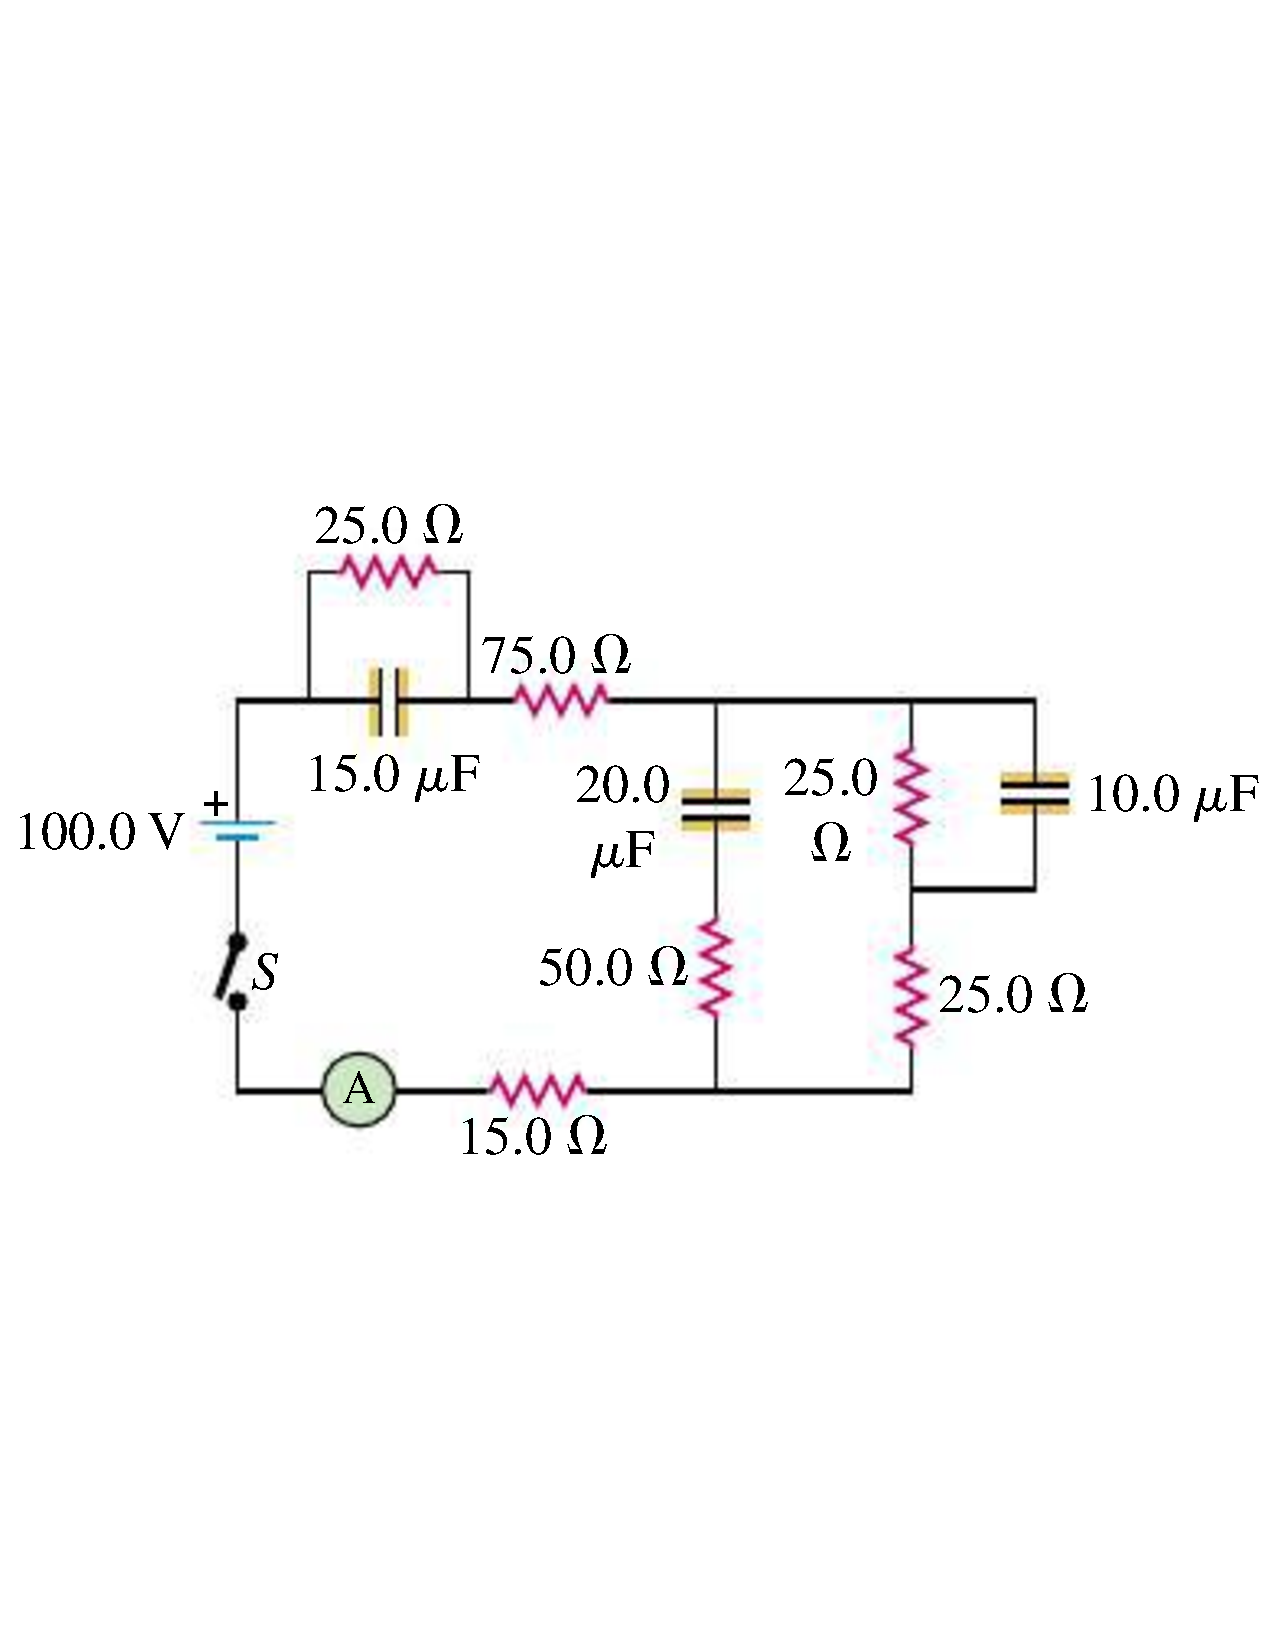
\includegraphics[scale=.31]{E26-47}
	\center \textbf{Figure E26.47}
\end{minipage}

\begin{solution}
	\begin{enumerate}
		\item Just after the switch is closed, there is no charge on any of the capacitors.  This means they act like a short in the circuit, so we can ignore any resistor that is in parallel with a capacitor.
		
		\vspace{1.5in}
		
		The \Sohm{50} and \Sohm{25} resistors are in parallel, and have the equivalent resistance $\Req$ given by
		\beq
			\frac{1}{\Req} = \frac{1}{\Sohm{50}} + \frac{1}{\Sohm{25}} = \frac{3}{50}\,\si{\per\ohm}
			\qimplies
			\Req = \frac{50}{3}\,\si{\ohm} = \Sohm{16.7}.
		\eeq
		
		\vspace{1.5in}
		
		The three resistances in series now give us the total resistance,
		\beq
			\Rtot = \Sohm{75.0} + \Sohm{16.7} + \Sohm{15.0}
			= \Sohm{106.7}.
		\eeq
		
		\vspace{1.5in}
		
		We can use Ohm's law to find the current through the equivalent resistance, which is the same as the ammeter reading:
		\beq
			\cE = I \Rtot
			\qimplies
			I = \frac{\cE}{\Rtot}
			= \frac{\Svolt{100.0}}{\Sohm{106.7}}
			= {\color{blue} \Samp{0.937}}.
		\eeq
		
		\item After $S$ has been closed for a very long time, the capacitors are completely charged and current cannot flow through them.  Therefore every capacitor acts like a break in the circuit, and we can adjust our diagram accordingly.
		
		\vspace{1.5in}
		
		This gives us five resistors in series, which have the equivalent total resistance
		\beq
			\Rtot = \Sohm{25.0} + \Sohm{75.0} + \Sohm{25.0} + \Sohm{25.0} + \Sohm{15.0}
			= \Sohm{165.0}.
		\eeq
		Once again, we use Ohm's law to find the ammeter reading:
		\beq
			I = \frac{\cE}{\Rtot}
			= \frac{\Svolt{100.0}}{\Sohm{165.0}}
			= {\color{blue} \Samp{0.606}}.
		\eeq
	\end{enumerate}
\end{solution}



\clearpage

\newcommand{\PcE}{P_\cE}
\newcommand{\dt}{\dd{t}}
\newcommand{\PR}{P_R}
\newcommand{\intoi}{\int_0^\infty}
\newcommand{\UC}{U_C}
\newcommand{\UcE}{U_\cE}
\newcommand{\UR}{U_R}

\paragraph{Problem 26.53}
\begin{problem}
	A capacitor with capacitance $C$ is connected in series to a resistor of resistance $R$ and a battery with emf $\cE$.  The circuit is completed at time $t = 0$.
	\begin{enumerate}
		\item In terms of $\cE$, $R$, and $C$, how much energy is stored in the capacitor when it is fully charged?
		\item The power output of the battery is $\PcE = \cE i$, with $i$ given by Eq.~\refeq{26.13}.  The electrical energy supplied in an infinitesimal time $\dt$ is $\PcE \dt$.  Integrate from $t = 0$ to $t \to \infty$ to find the total energy supplied by the battery.
		\item The rate of consumption of electrical energy in the resistor is $\PR = i^2 R$.  In an infinitesimal time interval $\dt$, the amount of electrical energy consumed by the resistor is $\PR \dt$.  Integrate from $t = 0$ to $t \to \infty$ to find the total energy consumed by the resistor.
		\item What fraction of the total energy supplied by the battery is stored in the capacitor?  What fraction is consumed in the resistor?
	\end{enumerate}
\end{problem}

\begin{solution}
	\begin{enumerate}
		\item In general, the potential energy $U$ stored in a capacitor is given by
		\beqn \tag{24.9}
			U = \frac{1}{2} C V^2,
		\eeqn
		where $C$ is the capacitor's capacitance and $V$ the potential difference between its plates.  When the capacitor its fully charged, the potential difference between its plates is the emf $\cE$.  So we have
		{\color{blue} \beq
			\UC = \frac{1}{2} C \cE^2.
		\eeq }
		
		\vfill
	
		\item In terms of the given quantities $\cE$, $R$, and $C$, the instantaneous current $i$ is given by
		\beq \label{26.13} \tag{26.13}
			i = \frac{\cE}{R} e^{-t / RC}.
		\eeq
		Plugging this in and integrating, the total energy supplied by the battery is
		\beq
			\UcE = \intoi \PcE \dt
			= \intoi \cE i \dt
			= \intoi \cE \frac{\cE}{R} e^{-t / RC} \dt
			= \frac{\cE^2}{R} \bigg[ - RC e^{-t / RC} \bigg]_0^\infty
			= \frac{\cE^2}{R} R C
			= {\color{blue} C \cE^2}.
		\eeq
		
		\vfill
		
		\item We just need to plug \refeq{26.13} in again and integrate to find the total energy consumed by the resistor:
		\begin{align*}
			\UR &= \intoi \PR \dt
			= \intoi i^2 R \dt
			= \intoi \left( \frac{\cE}{R} e^{-t / RC} \right)^2 R \dt
			= \frac{\cE^2}{R} \intoi e^{-2t / RC} \dt
			= \frac{\cE^2}{R} \left[ -\frac{RC e^{-2t / RC}}{2} \right]_0^\infty \\
			&= \frac{\cE^2}{R} \frac{RC}{2}
			= {\color{blue} \frac{1}{2} C \cE^2}.
		\end{align*}
		
		\vfill
		
		\item From (a) and (b), $\UC / \UcE = 1/2$, so {\color{blue} half} of the total energy supplied by the battery is stored in the capacitor.  From (b) and (c), $\UR / \UcE = 1/2$, so the other {\color{blue} half} of the total energy is consumed by the resistor.
	\end{enumerate}
\end{solution}



\clearpage

\begin{minipage}[l]{0.7\textwidth}
\paragraph{Problem 26.59}
\begin{problem}
	Calculate the currents $\Iq$, $\Iw$, and $\Ie$ indicated in the circuit diagram shown in \textbf{Fig.~P26.59}.
\end{problem}
\end{minipage}%
\hspace{0.05\textwidth}%
\begin{minipage}{0.25\textwidth}
	\center 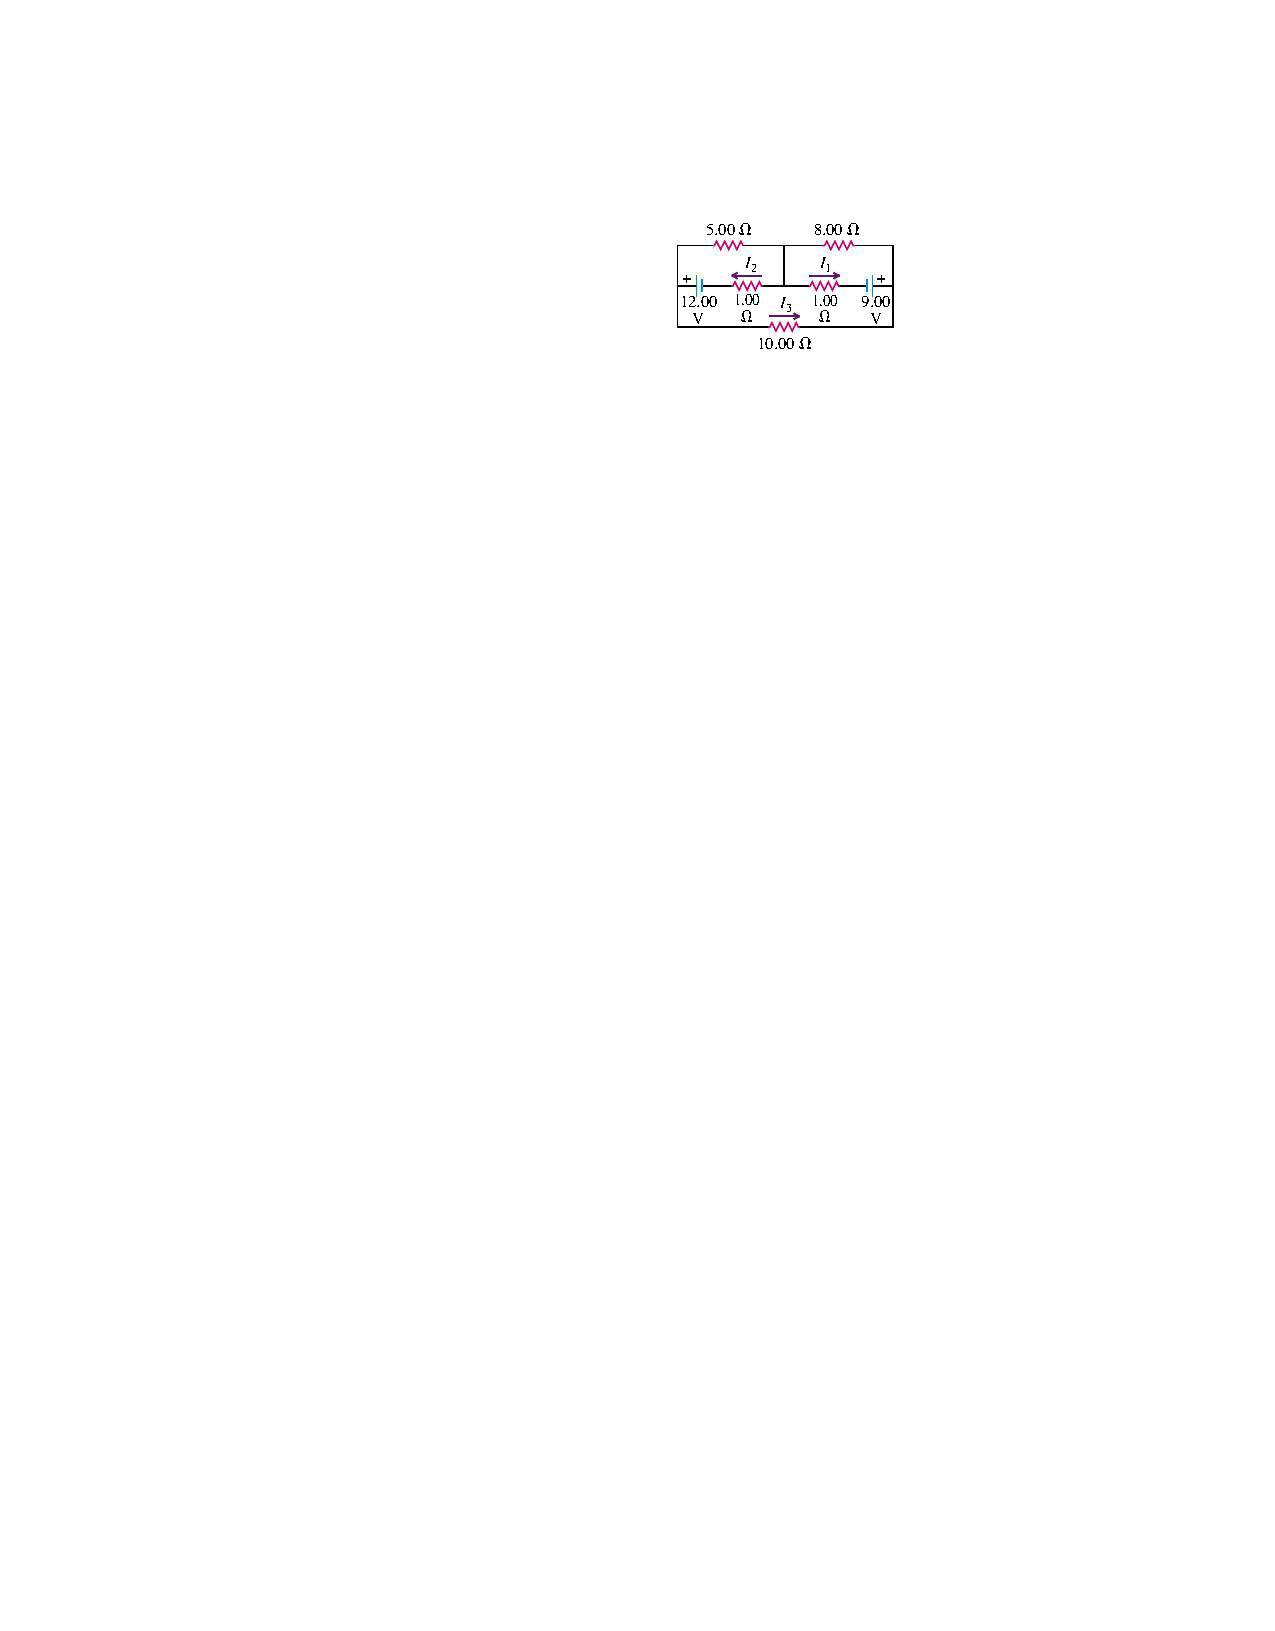
\includegraphics{P26-59}
	\center \textbf{Figure P26.59}
\end{minipage}

\begin{solution}
	This is another problem we can solve using Kirchhoff's rules.
	
	\begin{center}
		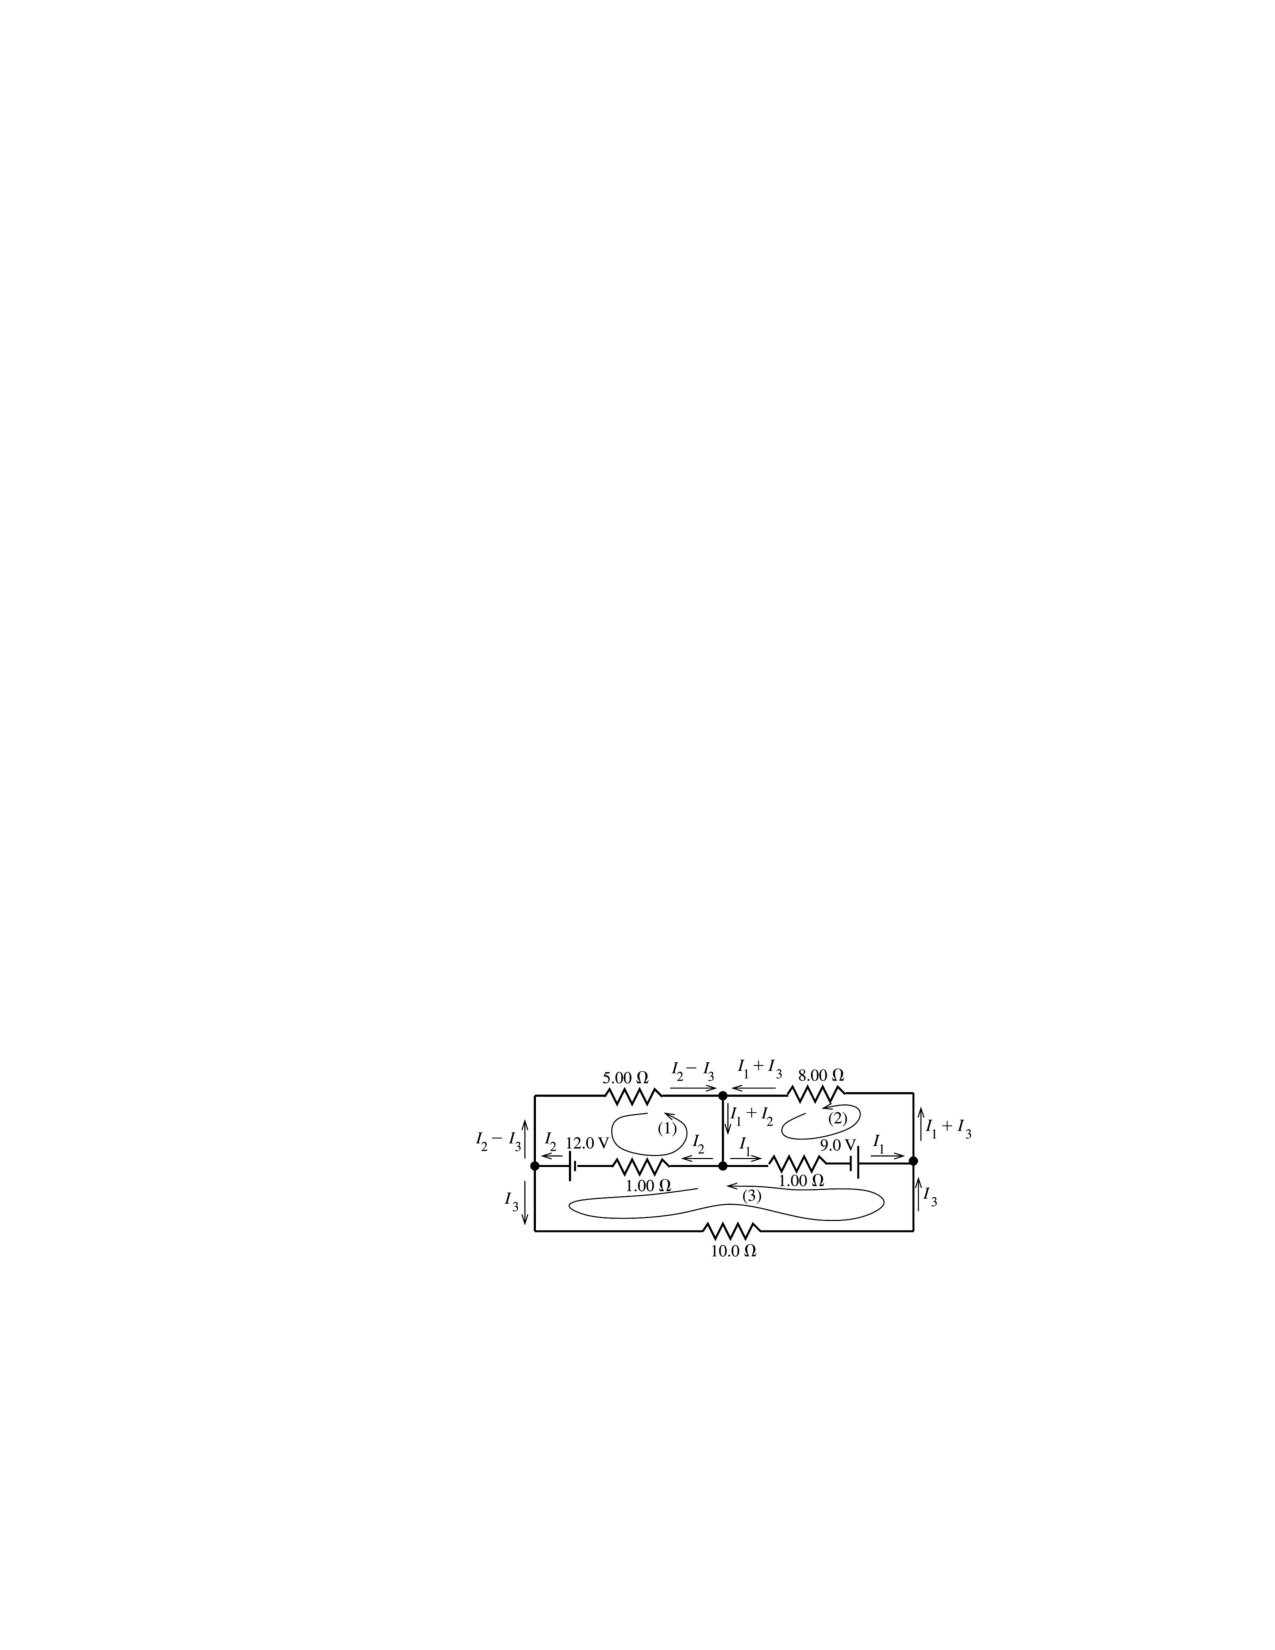
\includegraphics{A26-59}
	\end{center}
	
		The circuit has three loops, so we will need to use the loop rule three times.  But first we need to use the junction rule to find the current through the \Sohm{5} and \Sohm{8} resistors.  At the junction on the left (shown in red), we have
	\beq
		0 = \Iw - \Ie + I_{\Sohm{5}},
	\eeq
	which tells us the current through the \Sohm{8} resistor is
	\beqn \tag{A}
		I_{\Sohm{5}} = \Ie - \Iw,
	\eeqn
	meaning it is pointing away from the junction (as shown in the diagram) if $\Iw > \Ie$.
	
	At the junction on the right, we have
	\beq
		0 = \Iq + \Ie + I_{\Sohm{8}},
	\eeq
	which tells us the current through the \Sohm{8} resistor is
	\beqn \tag{B}
		I_{\Sohm{8}} = -\Iq - \Ie,
	\eeqn
	meaning it is pointing away from the junction as shown.
	
	Now we can apply the loop rule, moving counterclockwise from each battery.  For loop (1), we have
	\beq
		0 = -\Svolt{12} + (\Sohm{1}) \Iw + (\Sohm{5}) (\Iw - \Ie),
	\eeq
	which simplifies to
	\beqn \tag{1} \label{1}
		\Samp{12} = 6 \Iw - 5 \Ie.
	\eeqn
	For loop (2),
	\beq
		0 = \Svolt{9} - (\Sohm{8}) (\Iq - \Ie) + (\Sohm{1}) \Iq,
	\eeq
	which simplifies to
	\beqn \tag{2} \label{2}
		\Samp{9} = 9 \Iq + 8 \Ie.
	\eeqn
	For loop (3), let's start at the \Svolt{12} battery.  We find
	\beq
		0 = \Svolt{12} - (\Sohm{10}) \Ie - \Svolt{9} + (\Sohm{1}) \Iq - (\Sohm{1}) \Iw,
	\eeq
	which simplifies to
	\beqn \tag{3} \label{3}
		\Samp{3} = -\Iq + \Iw + 10 \Ie.
	\eeqn
	
	The loop rule has given us the system of three equations \refeq{1}, \refeq{2}, and \refeq{3},
	which you can solve using whatever method you like.  Since this system is more complicated than the system in \textbf{Exercise 26.26}, I prefer to use Gaussian elimination.  The matrix equation is
	\beq
		\mqty[ 0 & 6 & -5 \\
			9 & 0 & 8 \\
			-1 & 1 & 10 ]
			\mqty[ \Iq \\ \Iw \\ \Ie ]
			= \mqty[ 12 \\ 9 \\ 3 ],
	\eeq
	which can be solved as follows:
	\beq
		\begin{bmatrix}[c c c | c]
			0 & 6 & -5 & 12 \\
			9 & 0 & 8 & 9 \\
			-1 & 1 & 10 & 3
		\end{bmatrix}
		\sim
		\begin{bmatrix}[c c c | c]
			1 & 0 & 8/9 & 1 \\
			0 & 1 & -5/6 & 2 \\
			-1 & 1 & 10 & 3
		\end{bmatrix}
		\sim
		\begin{bmatrix}[c c c | c]
			1 & 0 & 8/9 & 1 \\
			0 & 1 & -5/6 & 2 \\
			0 & 1 & 98/9 & 4
		\end{bmatrix}
		\sim
		\begin{bmatrix}[c c c | c]
			1 & 0 & 8/9 & 1 \\
			0 & 1 & -5/6 & 2 \\
			0 & 0 & 211/18 & 2
		\end{bmatrix}
		\sim
		\begin{bmatrix}[c c c | c]
			1 & 0 & 0 & 179/211 \\
			0 & 1 & 0 & 452/211 \\
			0 & 0 & 1 & 36/211
		\end{bmatrix}.
		\eeq
		So we have {\color{blue}
		\begin{align*}
			\Iq &= \Samp{0.848} \text{ (to the right)}, &
			\Iw &= \Samp{2.14} \text{ (to the left)}, &
			\Ie &= \Samp{0.171} \text{ (to the right)}.
		\end{align*}}

\end{solution}


\end{document}